\documentclass[psamsfonts,onesided,10pt]{amsart}
\usepackage{goodstyle}


%opening
\title{HW 2 - Write Up}
\author{Robin Belton, Daniel Laden, Jiahui Ma,  Badr Zerktouni}

\begin{document}

\maketitle

\section{System Usage}

This system was written with Python version 3.7 and uses Iris Data csv located at \path{https://github.com/jiahuiblair/CSCI-550-HW2/iris.csv} 
to test clustering and assessment algorithms. All python functions and packages are included in the \path{main.py} file \todo{create this}

All functions can be run in the command line as follows:

\begin{description}
\item[Synthetic Data] To generate synthetic data where $(x,y)$ points are sampled from 
non-overlapping rectangular regions, run \textsc{SyntheticRectData}$(k,n,r)$ where $k$ is the 
number of points to sample from $n$ non-overlapping rectangular regions in $\mathbb{R}^2$. 
The noise parameter, $r$  is the number of noise points to add to the data that is not in the interior 
of any rectangular region. The output will be a data frame with attributes, `X', `Y', and `Label'. 
`X' and `Y' denote the $x-,y-$coordinates of the data point and the label denotes which rectangle 
the point was sampled from. A label of zero means the point is added noise.
\item[$k$-means] To cluster a two-dimensional dataframe $(x,y)$ through the $k$-means 
clustering algorithm, run \textsc{kmean}$(D,k,e)$ where $D$ is a three-dimensional dataframe with 
$x$, $y$ and a label column with NAN values, $k$ is the number of clusters specified by the user, 
and $e$ is the mean distance limitation between the most updated centroids and their previous 
centroids. The output of the \textsc{kmean}$(D,k,e)$ is a three-dimensional dataframe with $x$, $y$, 
and corresponding updated cluster label.
\item[DBSCAN] For our implimentation of DBSCAN the usual needed input of $\epsilon$ and MinPts. $\epsilon$ is the distance threshold value while MinPts is the needed neighbours in that distance to be considered a point of a cluster. We used Euclidean distance to calculate how far points are from each other, which may account for inconsistencies with base DBSCAN.
\item[Purity]  To compute the purity of a clustered dataset, $C$, to a given partition, $D$ run 
\textsc{Purity}$(D, C, n)$. $C$ and $D$ need to be data frames with 
attributes `X',  `Y', and `Label'. Additionally, this function is written for data that has been 
classified in three clusters where the labels of the clusters are either 1, 2, or 3. 
\item[Silhouette] To conduct internal assessment, run \textsc{internalassessment}$(D,k)$ 
where $D$ is a three-dimensional dataframe with $x$, $y$, and corresponding updated cluster 
labels, and $k$ is the number of clusters in the clustering. The output of this function is the 
average silhouette coefficient value of each points $(x,y)$ silhouette coefficients. 
\end{description}
 
\section{Example of Input/Output}
\begin{description}
\item[Synthetic Data] We run the SyntheticRectData for sampling 30 points from 3 
rectangular regions with 10 noise points. We also plot the results.
\begin{verbatim}
synth = SyntheticRectData(30,3,10)
plt.plot(synth['X'][0:29], synth['Y'][0:29], 'ro', #plot results
         synth['X'][30:59], synth['Y'][30:59], 'bo', 
         synth['X'][60:89], synth['Y'][60:89], 'go',
         synth['X'][90:99], synth['Y'][90:99], 'yo')
plt.show()   
\end{verbatim}
\begin{figure}[H]
    \centering
    {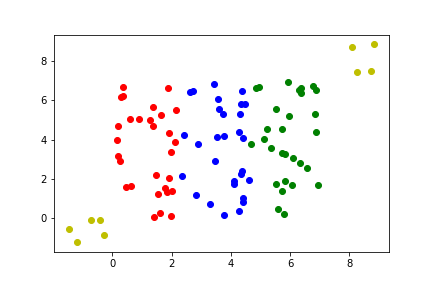
\includegraphics[width=.4\textwidth]{images/synth.png}} \\
    \caption{Plotting output of synth. Red, blue, and green represent the three rectangular regions. 
Yellow points are the added noise.}
\end{figure}
\item[$k$-means] Below we run the $k$-means algorithm with a dataframe (Sepal Length, Sepal Width, Label), $k$ equals to 3, and $e$ is 0.05. 
\begin{verbatim}
k=3
e=0.05
km=the dataframe
kmean(km,k,e)
\end{verbatim}
\begin{figure}[H]
    \centering
    {\includegraphics[width=.3\textwidth]{images/kmeans.png}} \\
    \caption{$k$-means output when applied to Sepal Length and Sepal Width of the Iris dataset.}
\end{figure}

\item[DBSCAN] Below we run the DBSCAN algorithm with a dataframe (Sepal Length, Sepal Width, Label), $\epsilon$ equals to 0.3, and $MinPts$ is 10. 
\begin{verbatim}
e=3
MinPts=10
sn=the dataframe
DBSCAN(sn,e,MinPts)
\end{verbatim}
\begin{figure}[H]
    \centering
    {\includegraphics[width=.3\textwidth]{images/kmeans.png}} \\
\end{figure}

\item[Purity] Below we first produce the ground truth data for the Iris dataset using Sepal Length 
and Sepal Width as the X and Y attributes. We then apply purity to the $k$-means output when $e=0.05$. 
\begin{verbatim}
D = iris[['Sepal Length', 'Sepal Width', 'Species']]
ground_truth = np.zeros((len(D.iloc[:,0]),3))
ground_truth[:,0] = D.iloc[:,0]
ground_truth[:,1] = D.iloc[:,1]
for i in range(len(D.iloc[:,0])):
    if D.iloc[i,2]=='Iris-setosa':
        ground_truth[i,2] = 1
    elif D.iloc[i,2]=='Iris-versicolor':
        ground_truth[i,2] = 2
    else:
        ground_truth[i,2] = 3
groundtruth = pd.DataFrame({'X':ground_truth[:,0], 'Y':ground_truth[:,1], 
                 'Label':ground_truth[:,2]})       
# Compute purity with Kmeans output, km (need to run k-means clustering function to get km)
Purity(groundtruth, km)
# output = 0.66
\end{verbatim}
\item[Silhouette] We run the internal assessment with the output dataframe from the 
$k$-means clustering algorithm where $k=3$. The ouput data frame from $k$-means is denoted by $km$.
\begin{verbatim}
internalassessment(km,k)
The Silhouette Coeff is 
0.27760826327927407
\end{verbatim}
\end{description}

\section{Exploring Datasets}
In this section we describe our findings from Part 4. We compared $k$-means to DBSCAN on the 
first two attributes (sepal length and sepal width) of the Iris dataset using the assessment 
measures of Purity and Silhouette. Furthermore, we explored 
how varying the number of sample points and noise points affect the purity of $k$-means. 

Below is a plot of how $k$-means clustered the Iris dataset with 3 clusters and $e=0.05$.
\begin{figure}[H]
    \centering
    {\includegraphics[width=.4\textwidth]{images/kmeans-clusters.png}} \\
    \caption{Plot $k$-means output when applied to Sepal Length and Sepal Width of the Iris dataset. Each color represents a different cluster.}
\end{figure}

A plot of the true classification of the Iris dataset is shown below.
\begin{figure}[H]
    \centering
    {\includegraphics[width=.4\textwidth]{images/groundtruth.png}} \\
    \caption{Plot of classification of Iris species based on Sepal Length and Sepal Width of the Iris dataset. Each color represents a different species.}
\end{figure}

Comparing the two plots, we see that $k$-means will never properly classify the three iris species 
since the red and green dots in the ground truth figure are ``well-mixed". Nevertheless, $k$-means 
does do a good job at classifiying the species represented by the blue dots. Using our assesment 
measures we found the puirty to be $0.666$ and silhouette coefficient to be $0.277608263$. 
Both these measures seem reasonable given the mixing of the red and blue in the ground truth plot.
Applying DBSCAN to the same dataset did not work as well. This is likely due to how there appears
 to be a uniform density of the points throughout. We were not able to find any parameters that 
produced three strong clusters. A radius of $\varepsilon = .3$  with minpts = 3 appears to 
produce two large clusters. However, we found that increasing the number of minpts increased 
the number of noise points, and increasing the radius started to collapse the clusters into one. 
We found DBSCAN to perform similarly on the synthetic data since the density of the 
points sampled is uniform throughout the rectangular regions, and the rectangular regions are 
close to one another.

Using our program to generate synthetic data that is drawn from three rectangles, we explored 
how increasing the sample size affected the purity of the $k$-means clustering. We only did this 
exploration for $k$-means since our purity function is only written for three clusters, and our 
DBSCAN output typically found more than three clusters. We found that 
keeping the noise constant while increasing the sample size did not appear to have an affect on 
purity. See Table 1. We repeated this small experiment several times and got similar results. 

\vspace{1ex}
\begin{center}
\begin{tabular}{ |c|c|c| } 
 \hline
\textbf{Sample} & \textbf{Noise} & \textbf{Purity}\\ 
40 & 5 & 0.648 \\ 
80 & 5 & 0.649 \\ 
120 & 5 & 0.611 \\ 
160 & 5 & 0.643 \\ 
200 & 5 & 0.648 \\ 
 \hline
\end{tabular}\\
\textbf{Table 1.} Purity assessments applied to $k$-means clustering of the synthetic data for 
different sample sizes.
\end{center}
\vspace{1ex}

Next, we used our program to generate synthetic data that is drawn from three rectangles to 
explore how increasing the noise affects the purity of the $k$-means clustering. We found that 
as noise increased, purity tended to decrease. See Table 2. Intuitively this makes sense since the 
noise points will be assigned to a cluster in $k$-means. However, by design, the noise points 
don't belong to any of the rectangles. Hence, the noise points will always negatively impact the purity measure. 

\vspace{1ex}
\begin{center}
\begin{tabular}{ |c|c|c| } 
 \hline
\textbf{Sample} & \textbf{Noise} & \textbf{Purity}\\ 
40 & 5 & 0.656 \\ 
40 & 10 & 0.59 \\ 
40 & 15 & 0.548 \\ 
40 & 20 & 0.59 \\ 
40 & 50 & 0.49 \\ 
 \hline
\end{tabular}\\
\textbf{Table 2.} Purity assessments applied to $k$-means clustering of the synthetic data for 
different amounts of noise.
\end{center}
\vspace{1ex}

In summary, we found $k$-means to work better on our synthetic data and Iris dataset than 
DBSCAN. This is because the true classification of these datasets formed convex sets where 
points were evenly distributed throughout. However, DBSCAN would perform better than 
$k$-means on a dataset that has non-convex clusters and where the true number of clusters is 
unknown. Additionally, we found that sample size did not impact $k$-means performance but 
noise did negatively impact $k$-means performance. Since DBSCAN is robust to noise, then we 
suspect that increasing the amount of noise would not negatively impact the purity measure of DBSCAN.

\end{document}
